\chapter{State of the Art}\label{ch:state-of-the-art}

\section{Problem 1 - Tactile Perception}\label{sec:lit-rev-problem-1}

% Based on the contact model categories described in \chapref{ch:modeling}, the most representative was chosen to be \gls{sf} models. 
% since these can provide descriptions of the contact surface shape, and thus enable the solving of the \gls{iep} by deriving surface features for pose estimation. Furthermore, these represent friction forces and moments that is needed to manipulate objects in hand and ensure force closure. 
% Within the category of \gls{sf} models, a method fit for this project's use case is to be chosen to solve problem~\ref{prob:1}. 
Of the contact models found during the literature review for solving problem~\ref{prob:1}
% \gls{sf} models can furthermore be divided up into 
four different categories were identified: \gls{aebm}, \gls{efm}, \gls{fem}~\cite{a-modified-elastic-foundation-contact-model-for-application-in-3d-models-of-the-prosthetic-knee} and \gls{ml} models. The different categories can be seen organized in \figref{fig:sf-categories} \medskip
%
\begin{figure}[h]
	\begin{small}
		\begin{center}
			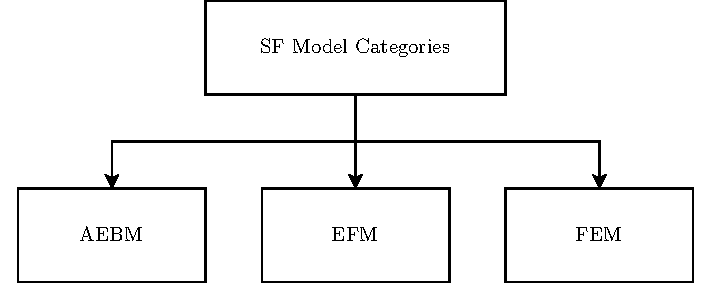
\includegraphics[width=0.8\textwidth]{chapters/state-of-the-art/fig/sf-categories.pdf}
		\end{center}
		\caption{Tree of methods for \gls{tp}.}
		\label{fig:sf-categories}
	\end{small}
\end{figure}

\gls{aebm} are theoretical formulations of elastic contact areas and the stresses on both the surfaces and the sub-surfaces of the contacting bodies. The first of such models was introduced by Heinrich Rudolf Hertz in \num{1882}~\cite{on-the-contact-of-rigid-elastic-solids-and-on-hardness} and is still used for simple contact cases. In the formulation of the Hertzian contact model, two assumptions are made: Objects in contact are made of linear elastic materials and only small contact deformations occur compared to the dimension of an object. However, robotic \gls{ee} fingertips are often made of non-linear elastic materials and for that reason, the basic Hertzian contact model does not represent the type of contact in this project~\cite[Chapter 37]{handbook-of-robotics}. To improve on the Hertzian model, a more general formulation can be made which extends the model from linear to nonlinear elastic contacts~\cite{modeling-of-contact-mechanics-and-friction-limit-surfaces-for-soft-fingers-in-robotics-with-experimental-results, the-haptic-and-perceptional-characteristics-of-an-anthropomorphic-curved-soft-finger-structure}. This power-law formulation subsumes the Hertzian contact theory while assuming a circular contact area. Other models have been purposed that combine the descriptions of both friction-contact and the shear-torsion as experienced by the bodies~\cite{the-sliding-of-robot-fingers-under-combined-torsion-and-shear-loading}. \medskip

However, to more accurately describe the contacts involving robot fingers, viscoelastic soft contact model appear more relevant due to such fingers often being made of materials that show viscoelastic properties e.g., rubber, silicone and polymers. Simple models such as  Kelvin-Voigt's~\cite{viscoelasticity} and Maxwell's~\cite{on-the-dynamical-theory-of-gases} models describe the interaction between strain and stress as a spring-damper system in a serial or in a parallel configuration respectively. Models which expand on this idea describe the reacting force as the product of the temporal and the elastic response while incorporating previous stress responses~\cite{mechanical-properties-and-active-remodeling-of-blood-vessels}. To simplify this formulation alternatives have been developed to assume no past stress~\cite{modeling-of-viscoelastic-contacts-and-evolution-of-limit-surface-for-robotic-contact-interface, characteristics-of-contact-and-limit-surface-for-viscoelastic-fingers, effect-of-layer-compliance-on-frictional-behavior-of-soft-robotic-fingers}. Upon these, more modern techniques have been developed which have seen use in similar use cases as the ones of interest in this project. 
% AEBM modern method 2 - A new algorithm for computing the indentation of a rigid body - reformulate - are frictionless MIM (matrix inversion).
One method attempts to expand the description of contacts between rigid indentors and elastic half-spaces, using the \gls{mim} as introduced by Kalker~\cite{on-the-contact-problem-in-elastostatics}, to viscoelastic half-spaces as well. Assuming the surfaces are frictionless, the relationship is described in terms of the pressure distribution, the resultant force on the indenter and the penetration~\cite{a-new-algorithm-for-computing-the-indentation-of-a-rigid-body-of-arbitrary-shape-on-a-viscoelastic-half-space}.
% AEBM modern method 3 - BC's Formulation
Attempts involving solutions to Boussinesq's problem for polynomial pressures acting over polygonal domains~\cite{a-general-approach-to-the-solution-of-boussinesqs-problem-for-polynomial-pressures-acting-over-polygonal-domains} have also been developed and modernized by combining it with Cerruti's solution~\cite{a-boussinesq-cerruti-solution-set-for-constant-and-linear-distribution-of-normal-and-tangential-load-over-a-triangular-area}. However due to numerical singularities being present, modifications are made to threshold the model. For a more complete description without singularities, Love's formulation has been added leading to a more accurate analytical representation but with the cost of an increased computational complexity~\cite{contact-modelling-and-tactile-data-processing-for-robot-skins}. For these Boussinesq-based approaches to be representative two assumptions are made 1) There exists a linear relationship between stress and strain, referred to as deformation, and 2) strains are infinitesimal~\cite[Chapter 6]{the-linearized-theory-of-elasticity}. \medskip

\gls{efm} are methods developed to build upon \gls{aebm} by allowing a simple discrete contact calculation in more general surface geometries. Here the deformable part of the contact is modeled as a layer over a rigid base with a series of discrete and independent springs in the contact normal. A widely used example of this method is Winkler's elastic foundation model~\cite{kl-johnson-and-contact-mechanics}, which has been used in structural engineering for modeling different properties of beams such as stability~\cite{stability-of-a-timoshenko-beam-resting-on-a-winkler-elastic-foundation}, vibrations and buckling~\cite{vibrations-and-buckling-of-a-beam-on-a-variable-winkler-elastic-foundation}. Other \gls{efm} methods have shown accurate modeling performance when applied within the field of medical engineering. Here a comparative study between \gls{aebm}, \gls{efm} and \gls{fem} demonstrate the suggested modified \gls{efm} performs better than the alternatives in 3D knee models when predicting prosthetic knee performance~\cite{a-modified-elastic-foundation-contact-model-for-application-in-3d-models-of-the-prosthetic-knee}. A different method attempts to attain vivo contact pressure predictions for improved knee replacement designs~\cite{experimental-evaluation-of-an-elastic-foundation-model-to-predict-contact-pressures-in-knee-replacements} Within the field of robotics \gls{efm} have provided solutions to problems such as slip~\cite{the-sliding-of-robot-fingers-under-combined-torsion-and-shear-loading}, compliance, sliding~\cite{quasistatic-manipulation-with-compliance-and-sliding, practical-force-motion-models-for-sliding-manipulation}, stiffness and contact mechanics~\cite{stiffness-and-contact-mechanics-for-soft-fingers-in-grasping-and-manipulation} of anthropomorphic grippers. One such method derives friction constraints based on general expressions for non-planar contacts of elastic bodies, where the local geometry and structure of the objects in contact are taken into account. Using these, a linear complementary problem is formulated and solved, resulting in the normal and frictional forces applied at each contact, as well as the relative velocity of the bodies involved~\cite{soft-finger-model-with-adaptive-contact-geometry-for-grasping-and-manipulation-tasks}. \medskip

\gls{fem} are popular general tools for solving \gls{pde}~\cite{history-of-finite-element-method:-a-review} and have seen contact applications in a wide range of engineering disciplines due to the assumptions made in \gls{aebm} and \gls{efm} not being applicable in these cases. A great number of these cases exist within the manufacturing industry~\cite{examples-of-fem-application-in-manufacturing-technology} whereas one example is the metal forming processes. Specifically, the estimation of wheel-rail profiles~\cite{contact-mechanics-analysis-of-measured-wheel-rail-profiles-using-the-finite-element-method} has been addressed using \gls{fem} due to the estimation of contacts over a greater surface is needed than what is assumed in \gls{aebm} and \gls{efm}. Other applications such as quality control through sliding wear estimation~\cite{simulating-sliding-wear-with-finite-element-method}, analysis of the responses of fully coupled thermo-elasto-plastic solids in contact~\cite{a-finite-element-procedure-for-the-analysis-of-thermo-mechanical-solids-in-contact} and performing diagnostics of failures in induction motors~\cite{induction-motors-fault-diagnosis-using-finite-element-method:-a-review}. Due to the complexity of modeling the contacts within robotics, \gls{fem} have become a popular choice and enabled tactile applications such as \gls{cobot} tactile skin for ensuring collaborative behavior when in contact~\cite{soft-robot-skin-with-conformal-adaptability-for-on-body-tactile-perception-of-collaborative-robots}, performance estimation of new tactile sensor technologies~\cite{design-and-experimental-research-of-robot-finger-sliding-tactile-sensor-based-on-fbg} and evaluating complex contact types by extending simulations and analysis systems~\cite{grasp-analysis-using-deformable-fingers}.
The modeling complexity has furthermore inspired using \gls{fem} as ground truth results when synthesizing \gls{ml} data in simulations for \gls{dl} models, which has enabled execution speeds \num{75} times greater than simply evaluating \gls{fem}~\cite{sim-to-real-for-robotic-tactile-sensing-via-physics-based-simulation-and-learned-latent-projections, interpreting-and-predicting-tactile-signals-via-a-physics-based-and-data-driven-framework, ground-truth-force-distribution-for-learning-based-tactile-sensing:-a-finite-element-approach}. \medskip

% introduction of ml methods %%%%%%%%%%%%%%%%%%%%%%%%%

The use of these \gls{ml} models has enabled realistic simulations of tactile sensor data. Current literature applies \gls{dl}-based approaches to simulate tactile sensor data for various tasks~\cite{more-than-a-feeling-learning-to-grasp-and-regrasp-using-vision-and-touch, single-grasp-object-classification-and-feature-extraction-with-simple-robot-hands-and-tactile-sensors}. For instance, simulating realistic tactile images from simulated contact depth to bridging
the reality gap for vision-based tactile sensing using a diffusion model~\cite{learning-to-read-braille:-bridging-the-tactile-reality-gap-with-diffusion-models}. Similarly, a \gls{cgan} has been used to simulate realistic tactile sensory data for use in tactile tasks~\cite{learning-to-read-braille:-bridging-the-tactile-reality-gap-with-diffusion-models}. Solutions using \gls{dl} models purely based on \gls{mlp} have been applied to enable real-time simulated realistic tactile data~\cite{simulation-of-the-syntouch-biotac-sensor}. \medskip

Given the methods presented above, the \gls{aebm} Boussinesq-Cerruti approach is considered along with the \gls{mlp} based \gls{dl} model. \medskip

Although the Boussinesq-Cerruti approach can produce precise tactile data and can be tailored to suit a particular case, it faces certain challenges. The model relies on certain assumptions regarding the materials in contact, including linear deformation and infinitesimal strains. Furthermore, evaluating the model requires complex calculations, such as multidimensional integrals, which significantly increase computation time and hinder real-time performance. In contrast to the transparency offered by the Boussinesq-Cerruti approach, the \gls{mlp} based approach is limited by the black-box nature of \gls{dl} models. Despite this drawback, \gls{mlp} based \gls{dl} models offer several benefits, such as low execution time and high adaptability to complex systems. Due to the high adaptability and option for real-time performance, the \gls{dl} model presented in~\cite{simulation-of-the-syntouch-biotac-sensor} is chosen to solve the \gls{tp} problem i.e. problem \ref{prob:1}.

% While the Boussinesq-Cerruti approach can provide high-quality tactile data with the option to modify and tune the model to fit the specific case, challenges arise as the model makes certain assumptions regarding the materials in contact. These assumptions include: the deformation is assumed linear along with the strains being infinitesimal. Additionally, when evaluating the model expensive computations are necessary such as multidimensional integrals, increasing the computation time and inhibiting real-time performance.

% Boussinesq-based approaches
% 	assumptions are not correct, execution time is slow.
% Machine learning 
% 	Due to these algorithms having a low execution time and high adaptability to complex systems
% For these Boussinesq-based approaches to be representative two assumptions are made 1) There exists a linear relationship between stress and strain, referred to as deformation, and 2) strains are infinitesimal

% tactile solutions for NN~\cite{touching-a-nerf-leveraging-neural-radiance-fields-for-tactile-sensory-data-generation}
% biotac_sim example
% One such example is the simulation of the SynTouch BioTac sensor when mounted on a Shadow Dexterous hand~\cite{simulation-of-the-syntouch-biotac-sensor}

% compare analytical and ml methods for pros and cons, choose which method is ideal for this case %%%%%%%%%%%%%%%%


% Due to these algorithms having . One such example is [insert machine learning achievements and how they are used in sensor simulation] \medskip

% Due to the accurate displacement representation and execution time, the machine learning-based approach is chosen.

% The contact model chosen for this project is the \gls{aebm} Love's formulation due to its capabilities of representing contact surface displacements with great precision~\cite{contact-modelling-and-tactile-data-processing-for-robot-skins}.

\section{Problem 2 - Pose Estimation}\label{sec:lit-rev-problem-2}

\gls{pe}, which involves determining the position and orientation of an object in 3D space, has been the subject of many research studies. The literature has identified two main categories of methods for solving this problem: those based on \gls{dl}, and those based on \gls{pcr}. \medskip

These can along with their subcategories be seen in~\figref{fig:pe-categories} as inspired by~\cite{a-comprehensive-survey-on-point-cloud-registration}.

\begin{figure}[h]
	\begin{small}
		\begin{center}
			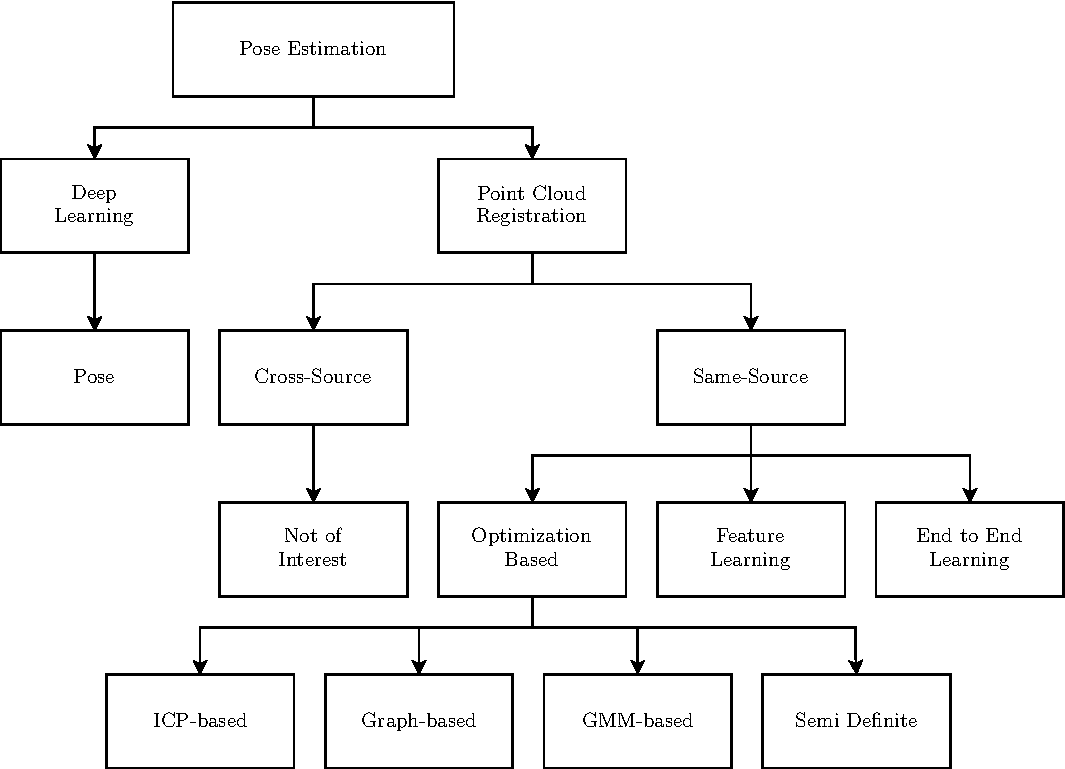
\includegraphics[width=0.8\textwidth]{chapters/state-of-the-art/fig/pe-categories-v3.pdf}
		\end{center}
		\caption{Tree of \gls{pe} methods. The categorization is inspired by~\cite{a-comprehensive-survey-on-point-cloud-registration}.}
		\label{fig:pe-categories}
	\end{small}
\end{figure}

Purely \gls{dl} based methods learn feature representations of input data, often in the form of images, and use them to estimate the subject's pose. This is commonly done in the context of human pose estimation~\cite{hands-deep-in-deep-learning-for-hand-pose-estimation, deeppose:-human-pose-estimation-via-deep-neural-networks, deeplabcut:-markerless-pose-estimation-of-user-defined-body-parts-with-deep-learning}. While these methods have shown extensive use in these cases, their applicability in this project is limited and thus excluded from consideration. \medskip

The other method group i.e. \gls{pcr} methods are separated into two subgroups: cross-source and same-source \gls{pc}s. Here cross-source refers to a \gls{pc} produced by combining information from sensors of different kinds e.g. visual- and tactile sensors, while same-source methods only produce \gls{pc}s based on information from the same kind of sensors e.g. only tactile sensors. 
While cross-source approaches have shown utility in an extensive range of applications~\cite{a-systematic-approach-for-cross-source-point-cloud-registration-by-preserving-macro-and-micro-structures,a-coarse-to-fine-algorithm-for-matching-and-registration-in-3d-cross-source-point-clouds,a-comprehensive-survey-on-point-cloud-registration} their applicability in this project is minimal, as purely tactile pose estimation is the problem of interest as presented in \chapref{ch:intro}. \medskip

\gls{pcr} methods from the same source data can be categorized into three sub-categories: end-to-end learning, feature-learning, and optimization-based methods. End-to-end learning-based methods use a neural network to estimate the transformation matrix that aligns two point clouds. Proposed solutions include using neural networks for scene completion to estimate the relative pose between RGB-D scans~\cite{extreme-relative-pose-estimation-for-rgb-d-scans-via-scene-completion}, learning registration patterns as parametric functions through a scan completion module and pairwise matching module~\cite{non-rigid-point-set-registration-networks}, and a fast feature-metric point cloud registration framework to minimize the feature-metric projection error without correspondences~\cite{feature-metric-registration:-a-fast-semi-supervised-approach-for-robust-point-cloud-registration-without-correspondences}.\medskip

In contrast, feature-learning methods use deep neural networks to learn robust feature correspondence searches, which are then used in estimation algorithms such as \gls{ransac}. In the literature, models have been developed to extract local geometric descriptors from RGB-D reconstructions~\cite{3dmatch:-learning-local-geometric-descriptors-from-rgb-d-reconstructions}, to learn globally informed 3D local feature descriptors~\cite{ppfnet:-global-context-aware-local-features-for-robust-3d-point-matching}, and to use siamese deep learning architectures with convolutional layers through a voxelized smoothed density value (SDV) representation~\cite{the-perfect-match:-3d-point-cloud-matching-with-smoothed-densities}. \medskip

% icp based methods
% In this paper we combine the Iterative Closest Point (ICP) and point-to-plane ICP algorithms into a single | Generalized-ICP algorithm

% 3 icp algorithm solutions


% 3 graph-based solutions 

% 3 gmm-methods

% semi-definite programming

% RCQP
% This allowed us to solve the original non-convex problem in a global fashion using its connection to the convex relaxation through duality theory


% we add GNC for robust outlier rejection

Lastly, registration methods based on optimization are employed to estimate the transformation matrix through two stages: correspondence searching and transformation estimation. Their goal is to minimize a cost function that gauges the dissimilarity between two point clouds. Within this category, there are four sub-categories identified: \gls{icp}-based, graph-based, \gls{gmm}-based, and \gls{sdp}-based methods. \medskip

Since the original proposal in 1992~\cite{a-method-for-registration-of-3-d-shapes} using point-to-point correspondences, \gls{icp}-based methods have evolved and incorporated different types of correspondences to improve performance. Examples include point-to-plane~\cite{object-modelling-by-registration-of-multiple-range-images} and plane-to-plane~\cite{generalized-icp}. Modern approaches also employ complementary methods such as point cloud filtering, adaptive fireworks algorithms, and KD-Trees~\cite{improved-iterative-closest-point-icp-3d-point-cloud-registration-algorithm-based-on-point-cloud-filtering-and-adaptive-fireworks-for-coarse-registration}. \medskip

% graph-based approaches 
The main idea of graph-based registration methods is to use a non-parametric model~\cite{a-review-of-point-set-registration:-from-pairwise-registration-to-groupwise-registration}. In this method, correspondences between two graphs are found by considering both the vertices and edges, making it an optimization problem~\cite{a-review-of-point-set-registration:-from-pairwise-registration-to-groupwise-registration}. To solve this optimization problem, there are two categories of graph-matching methods based on the objective functions' constraints: second-order and high-order methods~\cite{the-graph-matching-problem}. Second-order methods include \gls{csgm}~\cite{a-systematic-approach-for-cross-source-point-cloud-registration-by-preserving-macro-and-micro-structures}, which uses a linear program to solve the graph-matching problem and apply it to solve the cross-source point cloud registration task, \gls{fgm}~\cite{factorized-graph-matching} factorizes the large pairwise affinity matrix into smaller matrices and solves the graph-matching problem with a simple path-following optimization algorithm. Spectral graph~\cite{a-spectral-technique-for-correspondence-problems-using-pairwise-constraints} uses a spectral relaxation method to approximate the \gls{qap}, and \gls{sdp} relaxation is used to relax the non-convex constraint using a convex semi-definite. While higher-order graph matching provide methods for~\cite{probabilistic-graph-and-hypergraph-matching} design a probabilistic approach to solve the high-order graph-matching problem, while~\cite{a-tensor-based-algorithm-for-high-order-graph-matching} design a triangle similarity and convert the graph-matching problem into a tensor optimization problem. More recent work, such as~\cite{elastic-net-constraint-based-tensor-model-for-high-order-graph-matching} suggests an elastic net to control the trade-off between the sparsity and accuracy of the matching results by incorporating the Elastic-Net constraint into the tensor-based graph matching mode. \medskip

% gaussian mixture model
% \gls{gmm}-based methods attempt to convert the registration problem into a likelihood maximization problem for the input data, leading to the literature being focused on developing optimization strategies to maximize the likelihood and optimize the transformation matrix. One such example is~\cite{information-retrieval-for-music-and-motion} which introduces a \gls{cpd} in the form of a motion drift idea into the GMM framework by imposing constraints on transformation estimation. A different approach can be seen in~\cite{convex-hull-indexed-gaussian-mixture-model-ch-gmm-for-3d-point-set-registration} which combines the GMM with the convex hull, which is a tighter set of the original point set, to reduce computation complexity. Additionally, \gls{jrmpc}~\cite{a-generative-model-for-the-joint-registration-of-multiple-point-sets} approach registration as a clustering problem, where the transformation is optimized by solving the \gls{gmm}. More recently, \gls{deepgmr}~\cite{deepgmr:-learning-latent-gaussian-mixture-models-for-registration} has utilized deep learning to learn the correspondences between \gls{gmm} components and points. This enables the estimation of both the transformation and \gls{gmm} parameters in a single forward step.

\gls{gmm}-based methods commonly tackle the point cloud registration problem by transforming it into a likelihood maximization problem for the input data. This has resulted in the development of several optimization strategies aimed at maximizing the likelihood and optimizing the transformation matrix. For instance, a motion drift idea was introduced into the \gls{gmm} framework by~\cite{information-retrieval-for-music-and-motion} in the form of \gls{cpd} which imposes constraints on transformation estimation. In another approach,\cite{convex-hull-indexed-gaussian-mixture-model-ch-gmm-for-3d-point-set-registration} combines \gls{gmm} with the convex hull to reduce computation complexity. Furthermore, \gls{jrmpc}~\cite{a-generative-model-for-the-joint-registration-of-multiple-point-sets} cast registration as a clustering problem where the transformation is optimized by solving the \gls{gmm}. Recently, \gls{deepgmr}~\cite{deepgmr:-learning-latent-gaussian-mixture-models-for-registration} employed \gls{dl} to learn the correspondences between \gls{gmm} components and points, enabling the estimation of both the transformation and \gls{gmm} parameters in a single forward step. \medskip

Lastly, within \gls{sdp} different optimization groups exist, such as \gls{socp}, \gls{qp} and \gls{qcqp}. Due to the subject of interest being a rotation in SO(\num{3}), the constraints of the rotation matrix, i.e. quadratic constraints, must be respected. Because of this, the methods of \gls{qcqp} are of interest. \medskip

One such example provides estimates which are insensitive to a large fraction of spurious correspondences through decoupling the scale, rotation, and translation estimation. This decoupling enables the solving of these in cascade for the three transformations. The method is referred to as TEASER (Truncated least squares Estimation And SEmidefinite Relaxation), which solve large \gls{sdp} relaxations, and additionally comes with a second fast and certifiable algorithm, named TEASER++. To decrease execution time this method uses \gls{gnc} to solve the rotation subproblem and applies Douglas-Rachford Splitting to enable efficiently certify global optimality~\cite{teaser:-fast-and-certifiable-point-cloud-registration}. Secondly, Invariant-based Highly Robust Point Cloud Registration (IRON) applies a similar methodology as to TEASER, but instead applies RANSIC (RANdom Samples with Invariant Compatibility) to robustly estimates the scale between two sets of point clouds~\cite{iron:-invariant-based-highly-robust-point-cloud-registration}. Finally, \gls{rcqp} formulates a \gls{qcqp} problem with a full set of quadratic rotational constraints and obtains a Lagrangian dual relaxation, which empirically recovered a globally optimal solution in \SI{100}{\percent} of the tested cases, although why strong relaxation seems to hold has yet to be shown~\cite{convex-global-3d-registration-with-lagrangian-duality}. \medskip

Among the categories presented above, the ones of particular interest are optimization-based techniques due to their mature mathematical foundation and possible certifiable optimality and outlier rejection capabilities, and \gls{dl}-based techniques due to their adaptability and low execution time. While \gls{dl}-based methods can learn feature representations of point clouds and estimate the transformation between two point clouds, optimization-based approaches with outlier rejection can effectively handle noise and outliers in the data, which is a common problem within the \gls{pcr} problem. Due to this, the chosen method is the optimization based \gls{rcqp} method~\cite{convex-global-3d-registration-with-lagrangian-duality} with \gls{gnc} outlier rejection~\cite{graduated-non-convexity-for-robust-spatial-perception:-from-non-minimal-solvers-to-global-outlier-rejection}.



\section{Problem 3 - In-Hand Manipulation}\label{sec:lit-rev-problem-3}

Motion planning is a critical aspect of robot applications as it involves finding a path without collisions between two configurations. Planning dexterous manipulation paths can be a difficult endeavor due to the high dimension and computational complexity. During this literature review, the three main solution categories found were: kinodynamics, \gls{mpc} and \gls{rl}-based solutions, as seen in~\figref{fig:dm-categories}. \medskip

\begin{figure}[h]
	\begin{small}
		\begin{center}
			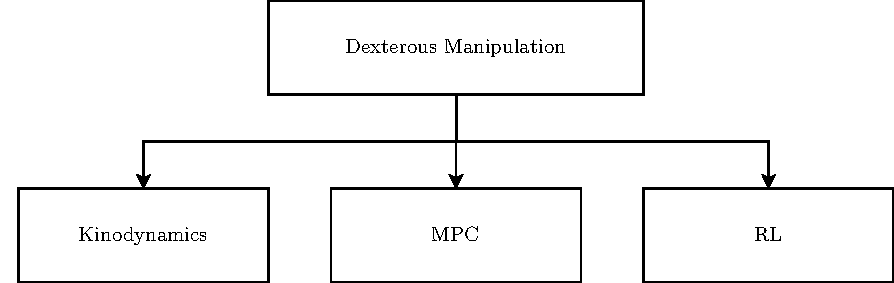
\includegraphics[width=0.8\textwidth]{chapters/state-of-the-art/fig/categories-dex-man.pdf}
		\end{center}
		\caption{Tree of methods for solving the in-hand manipulation problem.}
		\label{fig:dm-categories}
	\end{small}
\end{figure}

% kinodynamic
For kinodynamic motion planning to address the dexterous manipulation challenges, researchers have proposed probabilistic complete sampling-based kinodynamic motion planners like SST and SST*~\cite{asymptotically-optimal-sampling-based-kinodynamic-planning}. These planners utilize sampling-based techniques and probabilistic methods to generate collision-free paths in complex environments. Due to kinodynamics both searching in configuration space and its derivative, the problem becomes PSPACE-hard~\cite*{planning-algorithms}, indicating its great computational complexity. \medskip

% mpc
Despite their effectiveness, the complexity of the motion planning problem has led to the integration of motion planning algorithms with \gls{mpc}. By combining these two techniques, it becomes possible to avoid solving a boundary value problem~\cite{mpc-mpnet-model-predictive-motion-planning-networks-for-fast-near-optimal-planning-under-kinodynamic-constraints}, reducing the computational burden associated with kinodynamic motion planning. \medskip

% rl
Furthermore, to enhance performance, researchers have explored the combination of kinodynamic motion planning algorithms with \gls{rl}. This integration leverages the capabilities of \gls{rl} algorithms to learn from experience and improve the efficiency and quality of the generated motion plans~\cite{sampling-based-exploration-for-reinforcement-learning-of-dexterous-manipulation}. This however can become expensive due to the great search space, which has pushed the research into the applications of \gls{il} based \gls{rl}. One such example~\cite{dexmv:-imitation-learning-for-dexterous-manipulation-from-human-videos} which presents a novel framework for integrating expert demonstrations of dexterous manipulation into a wide range of \gls{rl} such as \gls{soil}, \gls{gail} and \gls{dapg}. \medskip

Overall, the field of motion planning has witnessed the development of various approaches to address the challenges posed by kinodynamic motion planning in high-dimensional spaces. From probabilistic complete sampling-based planners to the integration of \gls{mpc} and \gls{rl}, these advancements aim to enhance the efficiency, reliability, and adaptability of motion planning algorithms to support complex robot applications. \medskip

Due to the high flexibility and the results showed in~\cite{dexmv:-imitation-learning-for-dexterous-manipulation-from-human-videos}, which demonstrate applicable performance on a similar platform as the one chosen in this project, this method is chosen. Specifically the~\gls{dapg} \gls{rl} method, due to it showing the best overall results even in unseen cases.